\documentclass[UTF8]{ctexart}
\usepackage{geometry, CJKutf8}
\geometry{margin=1.5cm, vmargin={0pt,1cm}}
\setlength{\topmargin}{-1cm}
\setlength{\paperheight}{29.7cm}
\setlength{\textheight}{25.3cm}

% useful packages.
\usepackage{amsfonts}
\usepackage{amsmath}
\usepackage{amssymb}
\usepackage{amsthm}
\usepackage{enumerate}
\usepackage{graphicx}
\usepackage{multicol}
\usepackage{fancyhdr}
\usepackage{layout}
\usepackage{listings}
\usepackage{float, caption}

\lstset{
    basicstyle=\ttfamily, basewidth=0.5em
}

% some common command
\newcommand{\dif}{\mathrm{d}}
\newcommand{\avg}[1]{\left\langle #1 \right\rangle}
\newcommand{\difFrac}[2]{\frac{\dif #1}{\dif #2}}
\newcommand{\pdfFrac}[2]{\frac{\partial #1}{\partial #2}}
\newcommand{\OFL}{\mathrm{OFL}}
\newcommand{\UFL}{\mathrm{UFL}}
\newcommand{\fl}{\mathrm{fl}}
\newcommand{\op}{\odot}
\newcommand{\Eabs}{E_{\mathrm{abs}}}
\newcommand{\Erel}{E_{\mathrm{rel}}}

\begin{document}

\pagestyle{fancy}
\fancyhead{}
\lhead{姓名: 邓东宁}
\chead{数据结构与算法项目大作业}
\rhead{学号: 3230101177}
\cfoot{Dec.19th, 2024}

\section{项目简介}
简易的表达式计算器,支持输入有限位的正负实数,支持多重括号控制优先级、支持科学计数表示法。

\section{整体思路}
通过函数\verb|translate()|将人类惯用的中缀表达式翻译为方便机器阅读的后缀表达式,接着使用函数\verb|evalTranslation()|计算后缀表达式。用户端则通过\verb|expression_evaluator.h|开放的\verb|eval()|函数实现对中缀表达式的运算

\section{具体实现}
\subsection{函数translate()的实现}
依次遍历中缀表达式的字符,期间忽略空格并在遇到非法字符时退出报错。\\\\

若字符为数字类字符(指数字、小数点、作为负号的减号):
\begin{itemize}
    \item 直接把当前字符加入输出式
    \item 向后连续读取数字或小数点或字母\verb|e|,并也加入输出式。若加入的是\verb|e|,则还要再读取后面紧跟的数字
\end{itemize}
在这个过程中,为了确保一些减号能被正确识别为负号,需要用一个变量\verb|operandExpected|来指示,这个变量为\verb|True|等且仅当读到了运算符。\\\\

若字符为运算符类字符(指四则运算符外加一对圆括号):
定义一个堆栈结构\verb|operators|,用来缓存即将读到的运算符,并在恰当的时机把它们释放到输出式中
\begin{itemize}
    \item 若为左括号,则加入到\verb|operators|中,便于后续的右括号匹配
    \item 若为右括号,则向前遍历,依次把\verb|operators|缓存的运算符加入表达式,直到遇到左括号
    \item 若为运算符,则向前遍历,将高级或同级运算符依次加入到表达式,直到遇到比自己低级的运算符
\end{itemize}

最后还要遍历一次\verb|operators|,把剩下的低级运算符加入表达式。

\subsection{函数evalTranslation()的实现}
依然定义一个堆栈\verb|operands|用来缓存即将参与运算的对象(即数字和运算符)。\\
接着按照空格分隔后缀表达式,并依次遍历。\\
若遇到数字,则直接加入\verb|operands|中,同时使用\verb|std::stod()|识别科学计数法表示的数字。\\
若遇到符号,则将前两个数字依次弹出并按其在后缀表达式中的先后顺序进行二元运算,再讲结果加回\verb|operands|中便于后续继续运算。\\
读取完毕后,\verb|operands|会只剩下一个数字元素(若后缀表达式有效),则栈顶即结果。

\section{原理分析}
\subsection{后缀表达式}
在人类读取的中缀表达式中,我们需要首先识别最深层括号的位置,再根据运算符的优先级运算括号内表达式,再同理地依次向外层运算括号式,这个过程需要不断左右移动眼睛(对应机器的指针)去计算各部分,这个过程是代码难以复刻的,所以要让机器易读,最好的想法就是找到与中缀表达式等价的一种新的表达式,使得机器的指针(对应人类的眼睛)可以仅通过从左到右做连续单向移动,即可完成整个表达式的计算。\\
为了得到这样的表达式,我们要设法让数字成对出现,\textbf{它们之间涉及到的运算符按优先级紧随其后},在真正运算这样的表达式时,遇到数字即读取,遇到符号即运算前一对数字并把结果塞回去,最后所有符号都会因参与计算而消失,只留下一个数字,且这个数字是按照恰当的优先级算出的。\\
\subsection{优先级区分}
在上面的分析中,\textbf{加粗字体}的内容是本项目中最难想的一部分。为了方便想象,现假设存在足够多个不同优先级的运算符(加减乘除的推广),将中缀表达式中出现的第n个运算符$o_n$(可以有多个相同)按出现顺序赋予横坐标$n$,优先级为$a_n$,我将通过数列的特征辅助分析这个算法(如上图)。\\\\
\begin{figure}
    \centering
    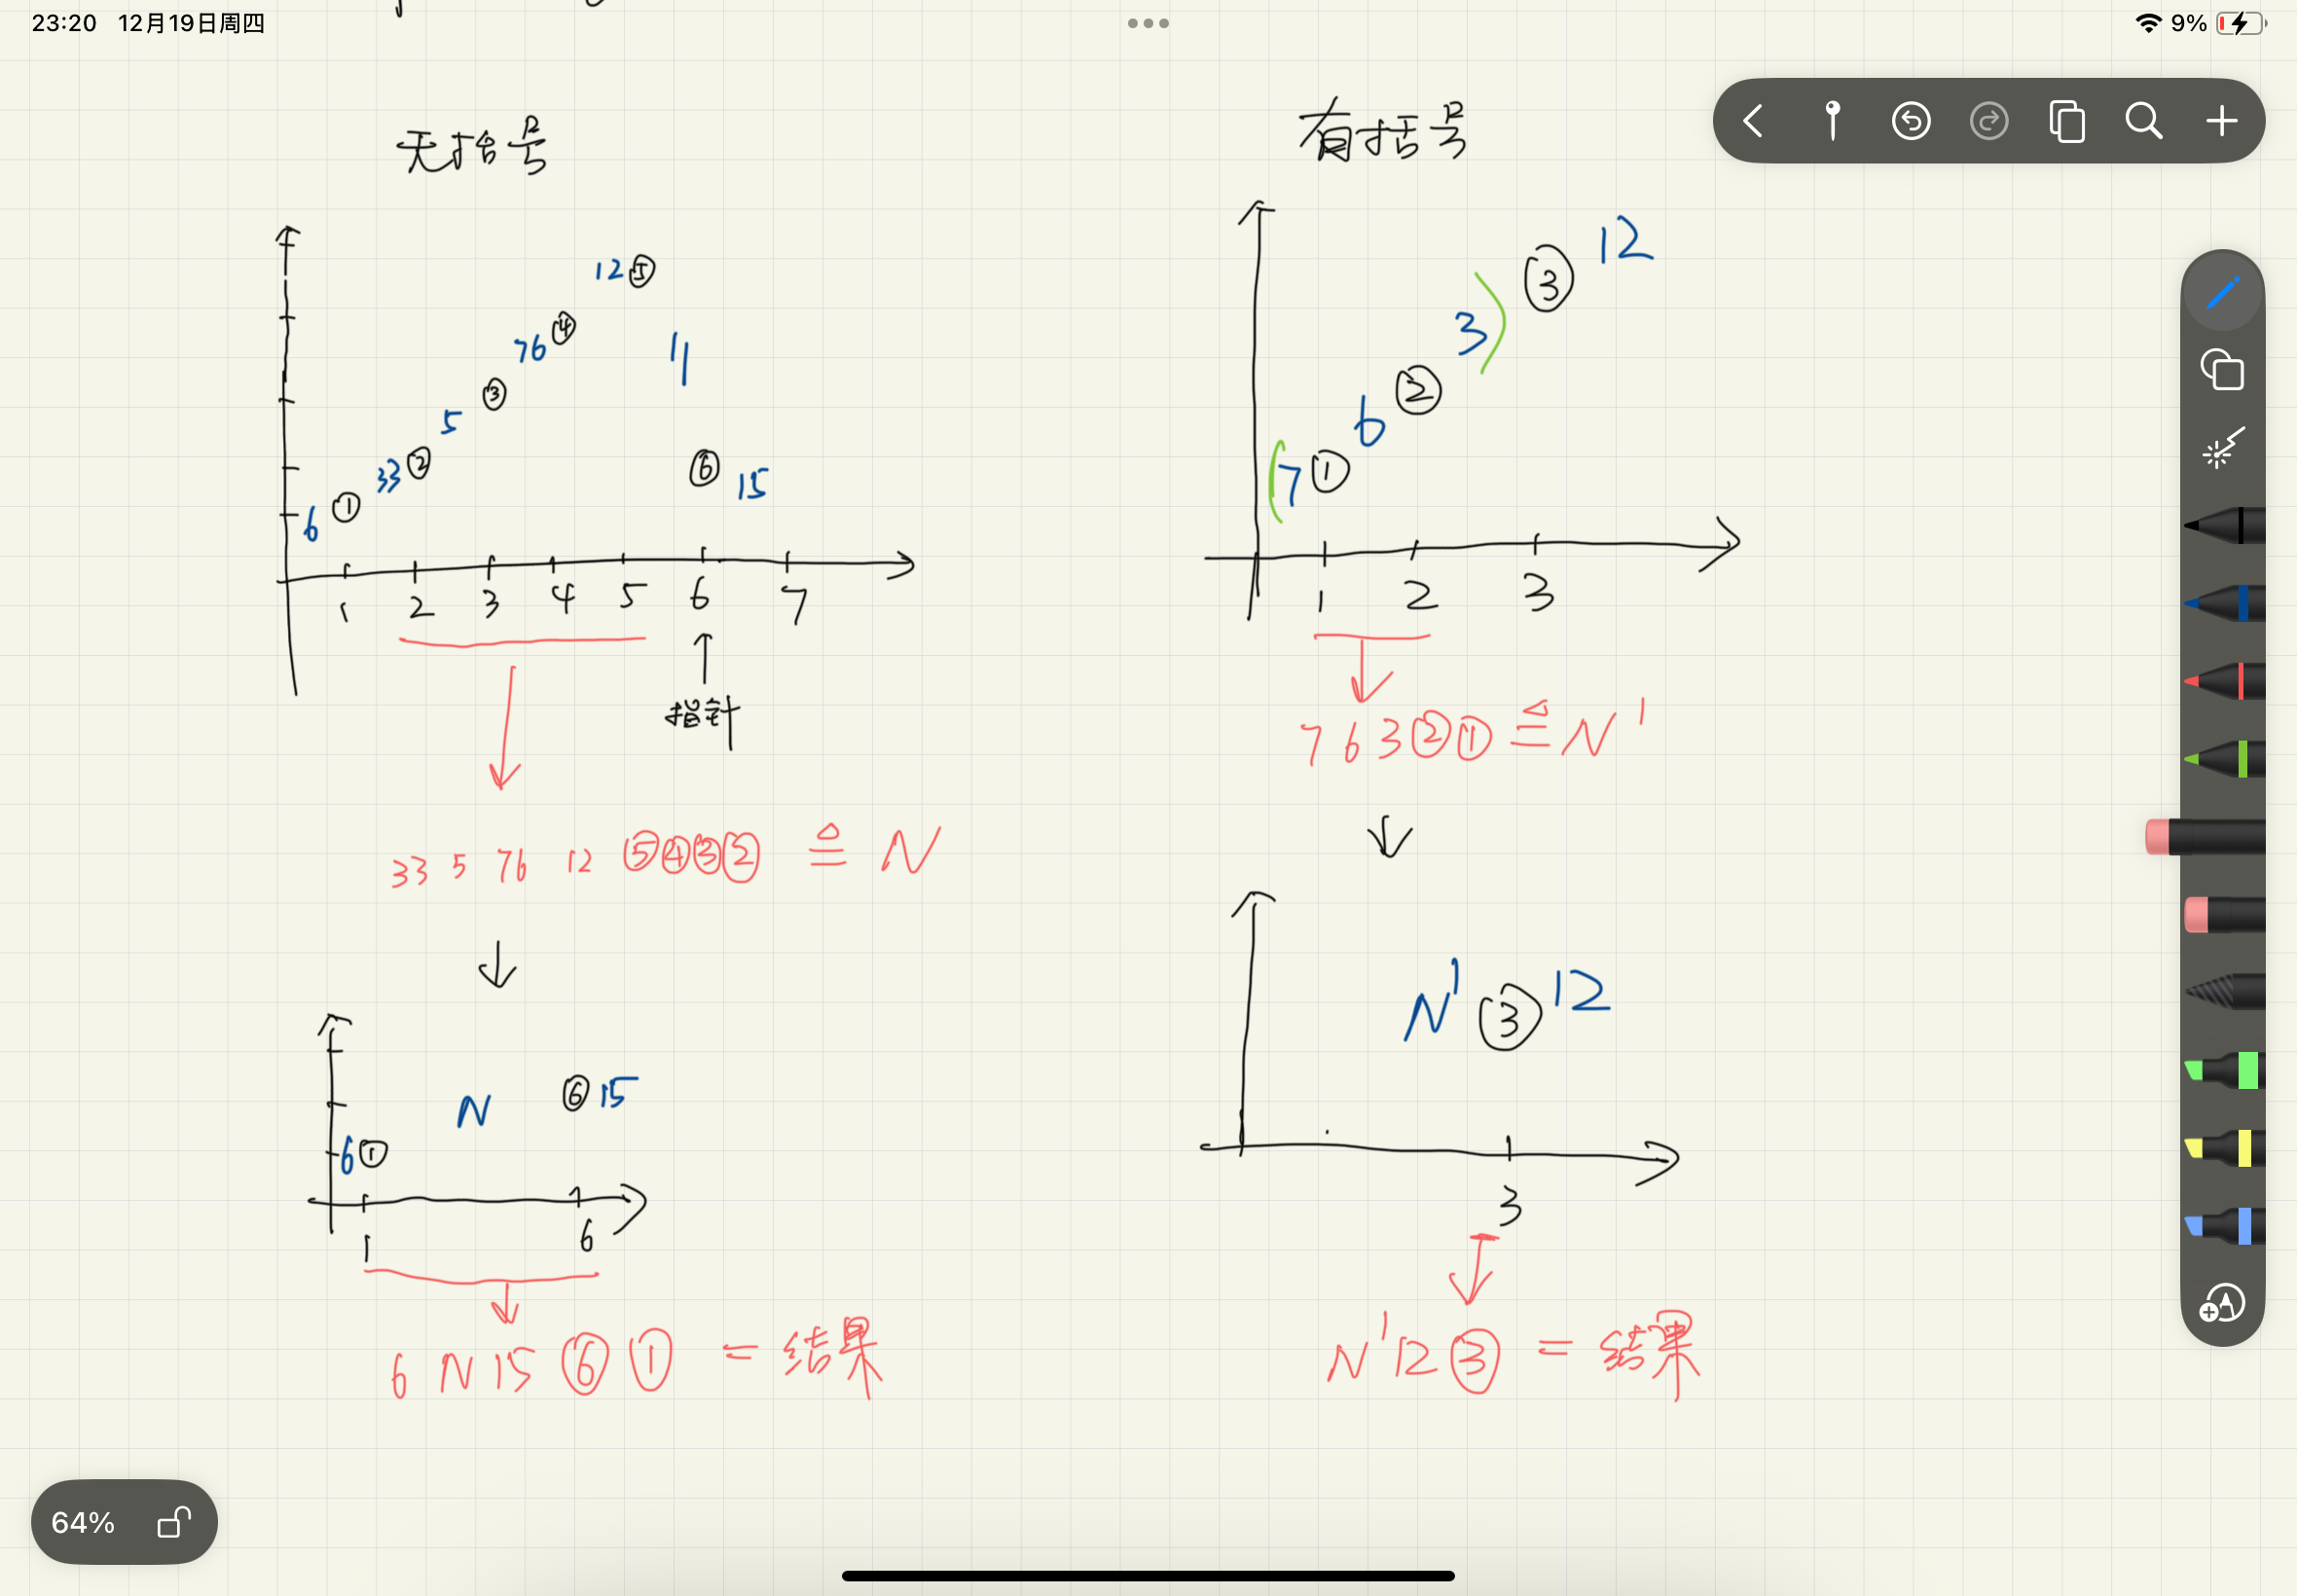
\includegraphics[width=0.5\linewidth]{analysis_figure.PNG}
    \caption{分析辅助用图,圈号代表第n个运算符,蓝色数字代表运算数     12.21补充:右图的括号最好应该画在坐标轴上因为括号优先级定义为0}
    \label{fig:enter-label}
\end{figure}
回顾我上面提到的\verb|translate()|实现过程:“若为运算符,则向前遍历,将高级或同级运算符依次加入到表达式,直到遇到比自己低级的运算符”\\
这个过程会维持数列的严格单调递增性——每当读取到一个破坏严格递增性的运算符时(即其指标为$n$),一定存在一个指标$m$,$m<n$,且$\forall m\leq i<n,a_i>a_n$,这个连续的子集自然也是严格单调递增的,这样只需直接把这个子集的运算符按倒序加入表达式,让优先级越高的运算符越贴近数字列,即可实现子结构运算的优先级区分,实际上在后缀表达式中,这个子结构产生的子表示式完全可以看做一个整体,即一个计算好的数。所以我们可以把这个头尖尖子集从原数列剔除(对应从\verb|operators|中移除元素),当做啥都没发生,继续读取,并按照上述规则维持严格递增性。处理完所有这样的子结构后,最后我们还会余下一个严格递增的子结构(当然也可能啥都不剩,对应\verb|operators|为空),再把这个余下的子集按倒序加入表达式,同理即可完成各子结构(都各当做一个算好的数)的运算优先级区分。\\\\

再来考察括号这一特殊符号怎么干涉上述过程:\\
返璞归真,回顾括号的作用:使得括号内部的子表达式的运算不受外部的任何运算符影响。
现在仅考虑整个表达式只有一层括号。\\
当读取到左括号时,仅是加入\verb|operators|,但啥也不干,等待后续读取到右括号来匹配以定位。\\
当读到潜在的低优先级运算符时,会回溯把运算符按逆序加入表达式,但遇到左括号后会强制停止,因为括号的优先级为0(这一点很重要)。这么做使得后续读到右括号时,括号内部的结构已经呈现了关于优先级的严格递增性。\\
当读取到右括号时,会直接回溯把括号内部剩下的运算符逆序加入表达式。\\
上述过程表明,括号的作用就是把包裹起来的子结构和其余结构独立开来,得到的后缀子表达式等价于一个算好的数,且这个算出来的数仅和括号内部的运算符有关,而不受到括号外部任何运算符的干扰。相应地,括号外部的运算也不会受到括号内部的干扰,毕竟内部产生的后缀表达式已经可以看成一个独立的数了,那么剩下的考虑过程遵循我上一大段说的即可。\\
对于多层括号的表达式,只需从最内层开始,向外依次考虑上述情形即可。\\

上述是对具有足够多不同优先级的运算符的分析,当优先级数量退化到2时,即本实例中$\times\ \div$的优先级为2,$+\ -$的优先级为1,上述分析也成立。与此同时,这也意味着这个算法也能处理运算符更丰富的表达式$\qedsymbol$ \\

\section{测试的结果}
\begin{table}[ht]
\centering
\begin{tabular}{|c|c|c|c|}  % 表示三列,使用竖线分隔
\hline  % 水平线
表达式 &测试目的& 结果 &符合预期\\  % 第一行内容
\hline
1+2*3 &简易表达式&  7&Y\\  % 第二行内容
\hline
(1+2)*3 &简易括号式&  9&Y\\  % 第三行内容
\hline
 1+(2+3)*4-5*(-6)+7/(8-9) &混合表达式&  44&Y\\
\hline
 (1+(2+(3+(4))))*5 &多重括号式&  50&Y\\
\hline
 1+(2*3+4)&多余括号式&  11&Y\\
\hline
 1.2*3.4 &小数运算& 4.08&Y\\
\hline
 1.2*-3.4 &负小数运算& -4.08&Y\\
\hline
 1+2e2 &科学计数法& 201&Y\\
\hline
 1+2e-1*5&负指数科学计数法& 2&Y\\
\hline
 1+2.3e4& 小数科学计数法& 23001&Y\\
\hline
 1+-1 &无括号表示负数& 0&Y\\\hline
 1--1&无括号表示负数& 2&Y\\\hline
 1 &单独数字& 1&Y\\\hline
 (((((1))))) &钻牛角尖& 1&Y\\\hline
 2.5cxk&拒绝非法字符& Error&Y\\
\hline
 1++1 &拒绝连用加号& Error&Y\\
\hline
 +1 &拒绝运算符开头& Error&Y\\
\hline
 1+ &拒绝未完待续& Error&Y\\
\hline
 1/0 &拒绝除以零& Error&Y\\
\hline
 (1+2+3 &拒绝括号不全& Error&Y\\
\hline
 (1+2+3))&拒绝括号不全& Error&Y\\
\hline
\end{tabular}
\caption{测试集}
\end{table}


\section{小结}
这份大作业消耗了我很多精力,想了很多,也错了很多,期间在代码方面也求助了多次AI,然后又独自花了许多时间绞尽脑汁理解过程并严谨地分析其可行性最后再把我所有的见解写到这篇report中,但总归,经过一番折腾,我对堆栈的理解确实大幅深化,通过在合适的时机\verb|pop|,可以合理地规划优先级,以实现不同的业务需求。最后预祝结课顺利,助教辛苦了!

\end{document}
